\chapter{Tests et qualité logicielle}

\section{Ma stratégie de tests}

Pour être sûr que l'application fonctionne correctement et reste maintenable, j'ai mis en place une stratégie de tests complète. Je suis la pyramide des tests : beaucoup de tests unitaires (rapides), moins de tests d'intégration, et encore moins de tests end-to-end (plus lents mais qui valident des parcours complets).

\subsection{Les différents types de tests}

\begin{itemize}
    \item \textbf{Tests unitaires :} Je teste chaque fonction ou composant isolément. Ils sont rapides et me permettent de détecter rapidement une régression.
    \item \textbf{Tests d'intégration :} Je vérifie que les différentes parties du système fonctionnent bien ensemble (par exemple, l'API avec la base de données).
    \item \textbf{Tests end-to-end (E2E) :} Je simule le parcours d'un utilisateur réel dans le navigateur, pour valider que tout fonctionne de bout en bout.
    \item \textbf{Tests de performance :} Je vérifie que l'application tient la charge et répond rapidement.
\end{itemize}

\begin{figure}[h]
    \centering
    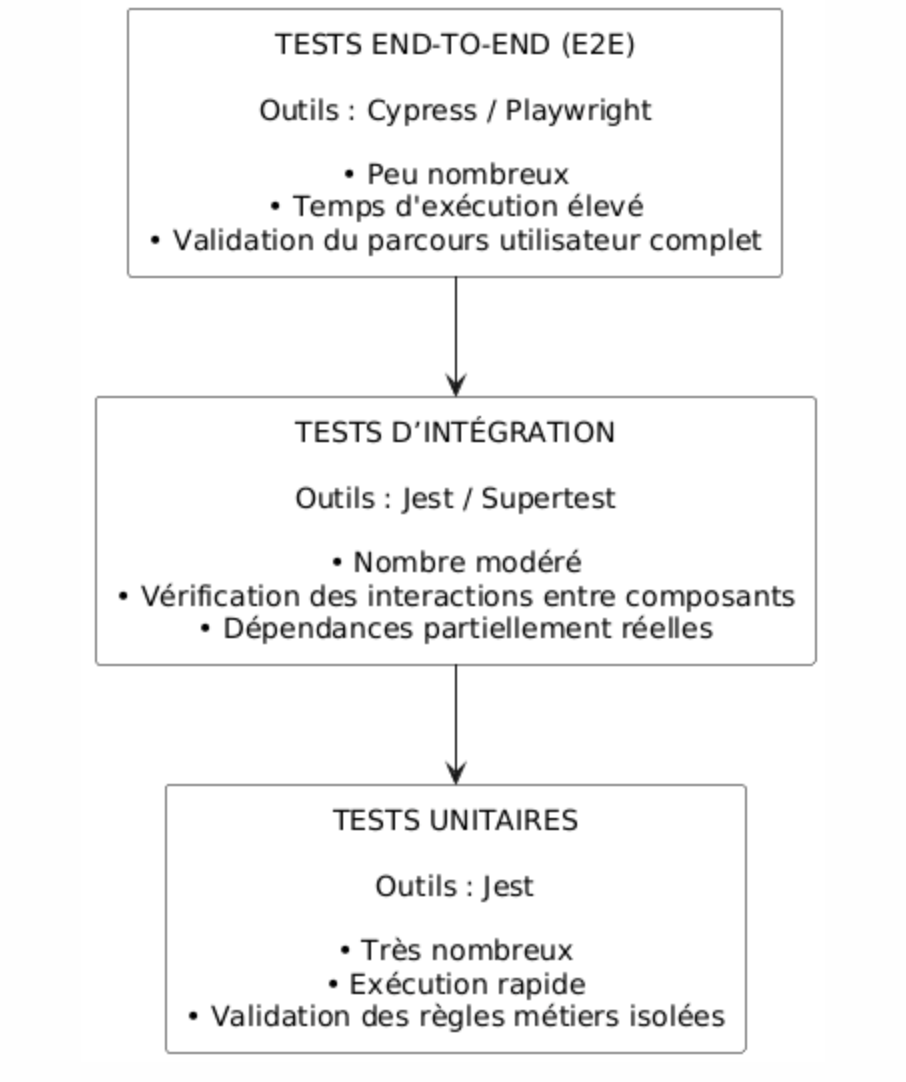
\includegraphics[width=0.6\textwidth]{assets/pyramide_test.png}
    \caption{La pyramide des tests : beaucoup de tests unitaires, moins de tests d'intégration, encore moins de tests E2E}
    \label{fig:pyramide}
\end{figure}

\subsection{Exemple de test unitaire}

Je teste une fonction du service de projet isolément, en "mockant" la base de données.

\begin{lstlisting}[language=JavaScript]
describe('ProjectService', () => {
  let projectService;
  let mockRepository;

  beforeEach(() => {
    // Je crée un faux repository pour ne pas toucher à la vraie base
    mockRepository = {
      create: jest.fn(),
      findById: jest.fn()
    };
    projectService = new ProjectService(mockRepository);
  });

  describe('createProject', () => {
    it('devrait créer un projet avec des données valides', async () => {
      // Données de test
      const projectData = {
        name: 'Test Project',
        description: 'Test Description',
        userId: 'user123'
      };
      
      // Je simule le comportement du repository
      mockRepository.create.mockResolvedValue({ 
        id: 'proj123', 
        ...projectData 
      });

      // J'exécute la fonction à tester
      const result = await projectService.createProject(projectData);

      // Je vérifie le résultat
      expect(mockRepository.create).toHaveBeenCalledWith(projectData);
      expect(result.id).toBe('proj123');
    });

    it('devrait rejeter un projet avec des données invalides', async () => {
      const invalidData = { name: '' }; // Nom vide = invalide

      await expect(projectService.createProject(invalidData))
        .rejects.toThrow('Le nom du projet est requis');
    });
  });
});
\end{lstlisting}

\subsection{Exemple de test d'intégration}

Je teste que mon API fonctionne correctement avec une vraie base de données (de test).

\begin{lstlisting}[language=JavaScript]
describe('API Projets', () => {
  let app;
  let authToken;

  beforeAll(async () => {
    // Je crée une instance de l'appli avec une base de test
    app = await createTestApp();
    // Je récupère un token d'authentification pour les tests
    authToken = await getTestAuthToken();
  });

  describe('POST /api/projects', () => {
    it('devrait créer un projet quand on est authentifié', async () => {
      const projectData = {
        name: 'Projet de test',
        description: 'Description test'
      };

      const response = await request(app)
        .post('/api/projects')
        .set('Authorization', `Bearer ${authToken}`)
        .send(projectData)
        .expect(201); // Je m'attends à un code 201 (créé)

      expect(response.body).toMatchObject({
        id: expect.any(String),
        name: projectData.name
      });
    });

    it('devrait refuser la création sans authentification', async () => {
      await request(app)
        .post('/api/projects')
        .send({ name: 'Test' })
        .expect(401); // Je m'attends à un code 401 (non autorisé)
    });
  });
});
\end{lstlisting}

\section{Tests de performance}

L'application doit rester rapide même quand plusieurs joueurs l'utilisent en même temps. J'utilise k6 pour simuler de la charge.

\subsection{Script de test de charge}

\begin{lstlisting}[language=JavaScript]
import http from 'k6/http';
import { check, sleep } from 'k6';

export let options = {
  stages: [
    { duration: '2m', target: 10 },  // Montée à 10 utilisateurs
    { duration: '5m', target: 50 },  // Montée à 50 utilisateurs
    { duration: '2m', target: 100 }, // Pic à 100 utilisateurs
    { duration: '5m', target: 50 },  // Redescente
    { duration: '2m', target: 0 },   // Arrêt
  ],
  thresholds: {
    http_req_duration: ['p(95)<500'], // 95% des requêtes < 500ms
  }
};

export default function() {
  // Connexion
  let loginResponse = http.post('http://localhost:3000/api/auth/login', {
    email: 'test@example.com',
    password: 'password123'
  });

  check(loginResponse, {
    'login status 200': (r) => r.status === 200,
  });

  if (loginResponse.status === 200) {
    const token = loginResponse.json('token');

    // Création d'un projet
    let projectResponse = http.post('http://localhost:3000/api/projects',
      JSON.stringify({ name: `Test ${__VU}` }),
      { headers: { 'Authorization': `Bearer ${token}` } }
    );

    check(projectResponse, {
      'project creation 201': (r) => r.status === 201,
    });
  }

  sleep(1);
}
\end{lstlisting}

\subsection{Résultats obtenus}

\begin{center}
\begin{tabular}{|l|l|l|l|}
\hline
\textbf{Métrique} & \textbf{Objectif} & \textbf{Mesuré} & \textbf{Statut} \\
\hline
Latence P95 & < 500ms & 320ms & ✅ \\
Débit & > 100 req/s & 150 req/s & ✅ \\
Taux d'erreur & < 1\% & 0.2\% & ✅ \\
CPU & < 80\% & 65\% & ✅ \\
Mémoire & < 2GB & 1.2GB & ✅ \\
\hline
\end{tabular}
\end{center}

\section{Qualité du code avec SonarQube}

Je ne suis pas tout seul pour juger de la qualité de mon code. SonarQube analyse automatiquement chaque commit et me remonte les problèmes.

\subsection{Ce que SonarQube surveille}

\begin{itemize}
    \item \textbf{Bugs :} Du code qui ne fait pas ce qu'il devrait.
    \item \textbf{Vulnérabilités :} Des failles de sécurité potentielles.
    \item \textbf{Code smells :} Du code mal écrit, difficile à maintenir.
    \item \textbf{Duplication :} Du code copié-collé (source d'erreurs).
    \item \textbf{Couverture de tests :} Est-ce que mes tests couvrent assez de code ?
\end{itemize}

\subsection{Mes résultats actuels}

\begin{center}
\begin{tabular}{|l|l|l|l|}
\hline
\textbf{Métrique} & \textbf{Objectif} & \textbf{Actuel} & \textbf{Statut} \\
\hline
Couverture de code & > 80\% & 85\% & ✅ \\
Duplication & < 3\% & 1.2\% & ✅ \\
Complexité cyclomatique & < 10 & 7.3 & ✅ \\
Maintenabilité & A & A & ✅ \\
Fiabilité & A & A & ✅ \\
Sécurité & A & A & ✅ \\
\hline
\end{tabular}
\end{center}

\subsection{Exemple de correction}

Quand SonarQube me signale un "code smell", je corrige. Exemple :

\begin{lstlisting}[language=JavaScript]
// AVANT : une fonction trop longue et qui fait trop de choses
const processUserData = (userData) => {
  const validatedData = validateUserData(userData);
  const processedData = transformUserData(validatedData);
  const enrichedData = enrichWithExternalData(processedData);
  const formattedData = formatForDatabase(enrichedData);
  const savedData = saveToDatabase(formattedData);
  const auditLog = createAuditLog(savedData);
  const notification = sendNotification(auditLog);
  return notification;
};

// APRÈS : je découpe en petites fonctions qui font une seule chose
const processUserData = (userData) => {
  const validatedData = validateUserData(userData);
  const processedData = transformUserData(validatedData);
  return saveUserData(processedData);
};

const saveUserData = (data) => {
  const enrichedData = enrichWithExternalData(data);
  const formattedData = formatForDatabase(enrichedData);
  const savedData = saveToDatabase(formattedData);
  auditUserAction(savedData);
  return savedData;
};
\end{lstlisting}

\subsection{Intégration dans GitHub Actions}

SonarQube est lancé automatiquement à chaque push :

\begin{lstlisting}[language=yaml]
name: Quality Gate
on: [push, pull_request]

jobs:
  quality:
    runs-on: ubuntu-latest
    steps:
      - uses: actions/checkout@v3
      - run: npm ci
      - run: npm test -- --coverage
      - name: SonarQube Scan
        uses: SonarSource/sonarqube-scan-action@v1
\end{lstlisting}

\section{Métriques Lighthouse}

Pour le frontend, j'utilise Lighthouse pour mesurer la qualité perçue par l'utilisateur.

\begin{itemize}
    \item \textbf{Performance :} 92/100 (objectif >90) - L'application est rapide.
    \item \textbf{Accessibilité :} 95/100 (objectif >90) - Elle est utilisable par tous.
    \item \textbf{Best Practices :} 88/100 (objectif >85) - Je suis les bonnes pratiques.
    \item \textbf{SEO :} 90/100 (objectif >85) - Elle est bien référençable.
\end{itemize}

\section{Ce que j'ai appris}

Mettre en place tous ces tests m'a pris du temps au début, mais c'est un investissement qui paie :

\begin{itemize}
    \item Je peux modifier mon code sans avoir peur de casser quelque chose d'autre (les tests me le diraient).
    \item La qualité est mesurable, je ne travaille plus "à l'instinct".
    \item Les utilisateurs beta ont trouvé beaucoup moins de bugs que sans tests.
    \item SonarQube m'a appris à écrire un code plus propre, même sur des choses auxquelles je n'avais pas pensé.
\end{itemize}